% !TEX root =  main.tex

%The high-level goal of \mEdhoc{} is to establish an authenticated security
%context for the \mOscore{} security protocol.
%
%To reach this goal,
%In this section, we provide an overview of the \mEdhoc{} protocol.
% For more details, we refer the reader to~\cite{selander-lake-edhoc-01}.
%To establish an authenticated security context for \mOscore,
The \mEdhoc{} specification~\cite{our-analysis-selander-lake-edhoc-00} uses
a three-message protocol structure, as
shown in Figure~\ref{fig:edhocFramework}.
%in the style of the \mNoise{} framework, outlined in
%
%The informal goal is to establish an \mOscore{} security context.
%
In the first message, the initiator $I$ sends to the responder $R$ an
ephemeral DH half-key \mGx{}, along with some parameters.
%
These parameters include proposed \mEdhoc{} authentication methods, proposed
cipher suites, connection identifier \mCi{} and optional application layer data
\mADone.
%
$R$ may reject the choice of the authentication methods
or cipher suites with an error message, leading to a negotiation across
multiple \mEdhoc{} sessions.
%an ordered list of supported cipher suites, and, in the \mMethod{} element, suggests
%authentication methods to be used.
%%
%\mT{R} may reject the choice of cipher suite, leading to a negotiation across multiple \mEdhoc{} sessions (see Section~\ref{sec:ciphersuiteNegotiation}), or that of the authentication methods.
%
In the second message, $R$ provides its ephemeral
DH half-key \mGy{} and its connection identifier \mCr, and authenticates itself
to $I$ by providing authentication data \mAuthr{}.
%
Finally, in the third message, $I$ authenticates itself
to $R$ by providing authentication data \mAuthi{}.
%
A party's authentication data consists of a MAC or a signature, depending on
authentication method used.
%

% KARL: Elaborating on this was requested by SSR reviewer #1
The connection identifiers \mCi{} and \mCr{}, described in Section 3.1 of the
\mSpec{}, deserve some elaboration.
%
The \mSpec{} describes these identifiers as not serving a security purpose for
\mEdhoc{}, but only as aiding message routing to the correct \mEdhoc{} processing
entity at a party.
%
Despite this, the \mSpec{} states that they may be used by \mOscore{}, or other
protocols using the established security context, without restricting how they
are to be used.
%
Because \mEdhoc{} may need them in clear-text for routing, \mOscore{} cannot
rely on them being secret.
%
Section 7.1.1 of the \mSpec{} requires the identifiers to be unique.
%
Uniqueness is defined to mean that $\mCi{} \not = \mCr{}$ for a given session
and the \mSpec{} requires parties to verify that this is the case.
%
The same section also require that \mOscore{} must be able to retrieve the
security context based on these identifiers.
%
The intended usage of \mCi{} and \mCr{} by \mOscore{} is not specific and
therefore it is not clear which properties should be verified.
%
We verify that the parties agree on the established values.
%

%We do not include \mCi, \mCr, and \mAD{} in our modelling here.
%As will be described below, 
%When authentication is based on
%a pre-shared key, the \mCredi{} and \mCredr{} credential identifiers are not
%used.
%
%Instead, a single identifier for the pre-shared key is transmitted in \mMsgone{}.
%
\begin{figure}
\centering
\tikzset{>=latex, every msg/.style={draw=thick}, every node/.style={fill=none,text=black}}
\begin{tikzpicture}
    \node (ini) at (0, 0) {Initiator ($I$)};
    \draw [very thick] (0, -0.25) -- (0,-2.2);
    \draw [very thick] (7, -0.25) -- (7,-2.2);
    \node (res) at (7,0) {Responder ($R$)};
    \msg{1em}{ini}{res}{\mMsgone: \mMethod, \mSuites, \mGx, \mCi, \mADone};
\msg{3em}{res}{ini}{\mMsgtwo: \mCi, \mGy, \mCr, [\mIdcredr, \mAuthr, \mADtwo]};
    \msg{5em}{ini}{res}{\mMsgthree: \mCr, [\mIdcredi, \mAuthi, \mADthree]};
    \draw [line width=1mm] (-0.75,-2.2) -- (0.75,-2.2);
    \draw [line width=1mm] (7-0.75,-2.2) -- (7+0.75,-2.2);
    \end{tikzpicture}
\caption{Structure of \mEdhoc{}: $[t]$ means $t$ is encrypted and integrity
protected. When a pre-shared key is used for authentication, its identifier is
included in \mMsgone{}.}
\label{fig:edhocFramework}
\end{figure}

%One of the driving design goals is to 
\mEdhoc{} accommodates three credential types
an party may use for authentication, 
%: certificates, private keys and static long-term DH keys. 
%
%The three authentication methods are based on 
namely digital signatures (\mSig), challenge-response signatures based on
static long-term DH keys (\mStat) and pre-shared keys (\mPsk).
%
%\pskstuff{and
%pre-shared symmetric keys (\mPsk)}.
%
%\pskstuff{While any combination of the \mSig{} and \mStat{} methods is possible,
%when \mPsk{} is used, both parties must use \mPsk{}.}
%
The initiator and responder are not required to use the same authentication
method.
%
Since both parties must use pre-shared key authentication if one of them does,
we have five combinations of authentication methods:
\mSigSig, \mSigStat, \mStatStat, \mStatSig{} and \mPskPsk.
%
We overload terminology and refer to these combinations of authentication methods as
\emph{methods} to follow the terminology in the \mEdhoc{}
\mSpec{}~\cite{our-analysis-selander-lake-edhoc-00}.
%
The individual authentication methods in each name denote the authentication
method used by the initiator and responder respectively.
%
We refer to a method where at least one party uses \mSig{}
(resp. \mStat{} or \mPsk{}) as a \mSig-based (resp. \mStat-based or \mPsk-based)
method.
%and similarly for \mStat{} and \mPsk.
%
The fields \mAuthi{} and \mAuthr{} are constructed in accordance with the
authentication method used.
%
For example, when authentication is based on digital signatures, the field is a
signed MAC.
%

%We first briefly discuss \mEdhoc's relations to the protocols on which it is
%based before providing details about the methods.
%

%-----------------------------------------------------------------------------
 
%\subsection{Relation to \mSigma, \mOptls{}, and \mNoise{}}
%\label{sec:relationsToOtherProtocols}
%We now present how \mEdhoc{} uses \mSigma, \mOptls{}, and \mNoise{} as
%cryptographic cores for various methods, and the ways in which it differs from them.
%\\
%%\mEdhoc{} uses existing academic protocols as cryptographic cores to
%%establish the session key.
%%
%%Being designed as an industrial standard, \mEdhoc{} specifies more details
%%on top of these cores, e.g., connection identifiers for message multiplexing,
%%encoding and application specific parameters to be negotiated.
%%
%
%%-----------------------------------------------------------------------------
%\runhead{\mSigma{}}
%%\subsubsection{\mSigma{}.}
%\label{sec:sigma}
%The \mSigSig{} method of \mEdhoc{} is closely modeled on the \mSigma{}
%variant that provides identity protection for the initiator~\cite{sigma}.
%%
%Some aspects differ though, e.g., \mSigSig{} uses Mac-then-Sign like
%\mTls{} instead of Sign-then-Mac. 
%%
%\\
%
%%----------------------------------------------------------------------------- 
%%\subsubsection{\mOptls{}.}
%\runhead{\mOptls{}}
%\label{sec:optls}
%The \mStat-based methods use challenge-response signatures based on static
%long-term DH keys, and proceed along the lines of
%\mOptls~\cite{DBLP:conf/eurosp/KrawczykW16}.
%%
%%The challenge-response signature works by one party sending a random challenge
%The challenge-response works as follows.
%%One party sends a random challenge
%Party $A$ sends a random challenge $r$
%%and an ephemeral DH half-key to a receiver.
%and an ephemeral DH half-key $e$ to a party $B$.
%%
%%The receiver mixes the DH half-key and the challenge with its secret static DH
%$B$ mixes $e$ and $r$ with its secret static
%long-term DH key $s$ to obtain a temporary key, which
%%
%is used to compute a MAC that is returned to 
%%the sender of the challenge.
%$A$.
%%
%%This authenticates the receiver to the sender, which is sufficient for \mOptls,
%This authenticates $B$ to $A$, which is sufficient for \mOptls, 
%because it only considers server authentication, where the server acts as $B$
%and the client as $A$.
%%
%The temporary key also affects the final session key.
%%
%
%In \mEdhoc, a party using the \mStat{} authentication method
%essentially acts as an \mOptls{} client and the peer as an \mOptls{}
%server.
%%
%However, unlike \mOptls{}, \mEdhoc{} requires mutual
%authentication~\cite{ietf-lake-reqs-04}.
%%
%\mStatStat{} can be thought of as interleaving two \mOptls{}
%runs, one initiated by each party, and then combining the resulting session key
%material.
%%
%Also, \mOptls{} uses the conservative security approach where $e$ and $r$
%are distinct elements, whereas \mEdhoc{} reuses the $e$ as the challenge $r$.
%%
%The latter can only weaken security.\\
%%
%
%%------------------------------------------------------------------------- sub
%%\subsubsection{\mNoise{}.}
%\runhead{\mNoise{}}
%The \mStatStat{} and \mPskPsk{} methods follow the \mNoise{}
%framework~\cite{perrin2016noise}.
%%
%\mNoise{} defines how to construct AKE protocols, using static long-term DH
%keys or pre-shared keys as credentials.
%%
%Its goal is to use so-called patterns to harmonize the many static long-term
%key DH-based AKE protocols, of which \mOptls{} is one.
%%
%\mNoise{} specifies how to derive keys, use transcript hashes to ensure
%authentication of the message flow etc.
%%among other things.
%%
%The \mNoise{} pattern closest to the \mStatStat{} method is called XX.
%%
%However, \mEdhoc{} does not use the functions of \mNoise{} exactly as
%prescribed.
%%
%It is thus not obvious that \mEdhoc{} automatically inherits
%the properties enjoyed by XX.
%%
%For example, according to \mNoise{}, the mixHash function is called on
%pre-message public keys during the initialization.
%%
%This would correspond to \mEdhoc{} computing a first intermediate transcript
%hash over those keys, which \mEdhoc{} does not do.
%%
%
%------------------------------------------------------------------------- sub
%\subsection{Methods of \mEdhoc{}}
%\label{sec:methods}
%Although \mCbor{} and \mCose{}~\cite{rfc8152} are important building blocks of
%\mEdhoc{}, and we use their terminology in our \mTamarin{} model to better
%reflect the \mSpec{}, our model does not cover the details of encoding and
%\mCose{} interfaces.
%
%Thus, we omit details about \mCbor{} and \mCose{}. 
%We refer the reader to~\cite{aead} for details about authenticated encryption with associated data (AEAD).
%
%All methods make use of a common key schedule, which we describe first.
%
%------------------------------------------------------------------------- sub
%\subsubsection{Key Hierarchy.}
%\runhead{Key Schedule}
%\label{sec:keyHierarchy}
At the heart of \mEdhoc{} is the key schedule depicted in
Figure~\ref{fig:kdfdiagram}.
%
\mEdhoc{} uses two functions from the \mHkdf{} interface~\cite{rfc5869} to derive keys.
%
\mHkdfExtract{} 
constructs uniformly distributed key material from random input and a salt,
while \mHkdfExpand{} generates keys from key material and a salt.
%
%The seeds are used to bind the key material and keys to certain parameters.
%

This key schedule is rooted in the ephemeral DH key \mGxy{}, the combination
of the two half-keys \mGx{}, \mGy{} and the corresponding secret half-keys $x$ and $y$.
%
From \mGxy{}, three intermediate keys \mPRKtwo, \mPRKthree{} and
\mPRKfour{} are derived during the course of protocol execution.
%
Each one of them is used for a specific message in the protocol, and from
these intermediate keys, encryption and integrity keys
(\mKtwoe, \mKtwom{}, \mKthreeae, and \mKthreem) for that message are derived.
%
The salt for generating \mPRKtwo{} is the empty string, or the pre-shared key in the case of \mPskPsk.%
%For \mPskPsk{}, the seed is the pre-shared key and for all other methods it is
%empty.
%

%In the 
%%\pskstuff{\mPskPsk{} and} 
%\mSigSig{} method, all three intermediate keys
%are the same, i.e., $\mPRKtwo{} = \mPRKthree{} = \mPRKfour$.
%%
%For the three \mStat-based methods, however, they differ.
%%
%This is because the intermediate key \mPRKthree{} is dependent on the static
%long-term key of the initiator if used (and \mPRKfour{} possibly also on the
%static long-term key of the responder).
%

Successful protocol execution establishes session key material.
%
%The key material is different for the different methods.
%
\mGxy{} is always part of the key material.
%
If the initiator uses the \mStat{} authentication method, so is
the initiator's public key \mGi{} raised to the power of $y$, a value which is
denoted \mGiy.
%
If the responder uses the \mStat{} authentication method,
the initiator's public key \mGr{} raised to the power of $x$, a value which is
denoted \mGrx{}, is part of the session key material.
%
From the session key material, a key exporter (\mEdhoc-Exporter) based on
\mHkdf{} is used to extract keys required for \mOscore{}.
%
%Figure~\ref{fig:kdfdiagram} shows an abstract description of the key schedule.
%

\begin{figure}[h]
\centering
\scalebox{.785}{
% !TEX root =  edhocProtocol.tex
% Start the picture
\begin{tikzpicture}[%
    >=latex,              % Nice arrows; your taste may be different
    start chain=going below,    % General flow is top-to-bottom
    node distance=10mm and 60mm, % Global setup of box spacing
    every join/.style={norm},   % Default linetype for connecting boxes
    ]
% ------------------------------------------------- 
% A few box styles 
% <on chain> *and* <on grid> reduce the need for manual relative
% positioning of nodes
\tikzset{
terminput/.style={rounded corners, text width=6em},
term/.style={rounded corners},
  base/.style={draw, thick, on chain, on grid, align=center, minimum height=6ex},
  prk/.style={base, draw=Red3, fill=Red3!25, rectangle, text width=4em},
  %hkdfext/.style={base, draw=Green3, fill=Green3!25, isosceles triangle, isosceles triangle apex angle=60, anchor=base, shape border rotate=-90, text width=6em},
  hkdfext/.style={base, draw=Green3, fill=Green3!25, rectangle, text width=8em},
  %hkdfexp/.style={base, draw=orange, fill=orange!50, isosceles triangle, isosceles triangle apex angle=60, anchor=base, shape border rotate=-90, text width=6em},
  hkdfexp/.style={base, draw=orange, fill=orange!50, rectangle, text width=8em},
  keyb/.style={base, draw=Blue3, fill=Blue3!25, rectangle, text width=4em},
  % -------------------------------------------------
  norm/.style={->, draw, Blue3},
}
% -------------------------------------------------
% Start by placing the nodes
\node [prk] (p0) {$g^{xy}$};
\node [hkdfext, join] (h1) {\mHkdfExtract};
\node [prk, join] (p2) {\mPRKtwo};
\node [hkdfext, join] (h3) {\mHkdfExtract};
\node [prk, join] (p3) {\mPRKthree};
\node [hkdfext, join] (h5) {\mHkdfExtract};
\node [prk, join] (p4) {\mPRKfour};

\node [hkdfexp, shape border rotate=180, left= 3cm of p4] (h6) {\mHkdfExpand};
\node [keyb, join, left=3cm of h6] (k3) {\mKthreem};

\node [hkdfexp, shape border rotate=180, left= 3cm of p3] (h4) {\mHkdfExpand};
\node [keyb, join, left=3cm of h4] (k2) {\mKtwom};

\node [hkdfexp, shape border rotate=180, left= 3cm of p2] (h2) {\mHkdfExpand};
\node [keyb, join, left=3cm of h2] (k1) {\mKtwoe};

\node [hkdfexp, shape border rotate=180, below= 1cm of h4] (h8) {\mHkdfExpand};
\node [keyb, below=1cm of k2] (k2b) {\mKthreeae};
%\node [draw=none, fill=none, below=0.5cm of h4] (dummy) {};

\draw [->, norm] (p3.south) -- ++(0,-0.58) -- (h8);
\draw [->, norm] (h8) -- (k2b);
\draw [->, norm] (p2) -- (h2); 
\draw [->, norm] (p3) -- (h4); 
\draw [->, norm] (p4) -- (h6);
%\node [term, fill=Green3!25, below = -1.3cm of h1] (h1name) {\mHkdfExtract};
%\node [term, left = 1cm of h1name] (u1) {H1};
%\draw [->, dotted, shorten >=1mm] (u1) -- (h1name);
\node [terminput, right = 1cm of h1] (u1) {Initial salt};
\draw [->, dotted, shorten >=1mm] (u1) -- (h1);

%\node [term, fill=Green3!25, below = -1.3cm of h3] (h3name) {\mHkdfExtract};
%\node [term, left = 1cm of h3name] (u2) {H2};
%\draw [->, dotted, shorten >=1mm] (u2) -- (h3name);
\node [terminput, right = 1cm of h3] (u2) {Additional input};
\draw [->, dotted, shorten >=1mm] (u2) -- (h3);

\node [terminput, right = 1cm of h5] (u3) {Additional input};
\draw [->, dotted, shorten >=1mm] (u3) -- (h5);


%\node [term, fill=orange!50, below = -0.9cm of h2] (h2name) {\mHkdfExpand};
%\node [term, above = 1cm of h2name] (u3) {H3};
%\draw [->, dotted, shorten >=1mm] (u3) -- (h2);
\node [term, above = 1cm of h2] (u4) {\mTHtwo};
\draw [->, dotted, shorten >=1mm] (u4) -- (h2);

%\node [term, fill=orange!50, below = -0.9cm of h4] (h4name) {\mHkdfExpand};
%\node [term, above = 1cm of h4name] (u5) {H5};
%\draw [->, dotted, shorten >=1mm] (u5) -- (h4);
\node [term, above = 1cm of h4] (u5) {\mTHtwo};
\draw [->, dotted, shorten >=1mm] (u5) -- (h4);

\node [term, above = 0.7cm of h6] (u6) {\mTHthree};
\draw [->, dotted, shorten >=1mm] (u6) -- (h6);
\draw [->, dotted, shorten >=1mm] (u6) -- (h8);
%
% ------------------------------------------------- 
% 
%\path (h2.east) to node [near start, yshift=1em] {$n$} (c3); 
%  \draw [o->,lccong] (h2.east) -- (p8);
%\path (p3.east) to node [yshift=-1em] {$k \leq 0$} (c4r); 
%  \draw [o->,lcnorm] (p3.east) -- (p9);
% -------------------------------------------------
% 
%\path (h1.east) to node [near start, yshift=1em] {$n$} (c1); 
%  \draw [o->,lcfree] (h1.east) -- (c1) |- (p4);
%\path (h3.east) -| node [very near start, yshift=1em] {$n$} (c1); 
%  \draw [o->,lcfree] (h3.east) -| (c1);
%\path (p3.west) to node [yshift=-1em] {$k>0$} (c4); 
%  \draw [*->,lcnorm] (p3.west) -- (c4) |- (p3);
%\path (h4.east) -| node [very near start, yshift=1em] {$n$} (c6); 
%  \draw [o->,lcfree] (h4.east) -| (c6); 
%\path (h5.east) to node [near start, yshift=1em] {$n$} (c6); 
%  \draw [o->,lcfree] (h5.east) -| (c7); 
%\path (p4.east) to node [yshift=-1em] {$k \leq 0$} (c7); 
%  \draw [o->,lcfree] (p4.east) -- (c7)  |- (p9);
%\path (p4.west) to node [yshift=-1em] {$k>0$} (c5); 
%  \draw [*->,lcfree] (p4.west) -- (c5) |- (p5);
% -------------------------------------------------
% A last flourish which breaks all the rules
%\draw [->,MediumPurple4, dotted, thick, shorten >=1mm]
%  (p9.south) -- ++(5mm,-3mm)  -- ++(27mm,0) 
%  |- node [black, near end, yshift=0.75em, it]
%    {(When message + resources available)} (p0);
% -------------------------------------------------
\end{tikzpicture}
% =================================================

}
\caption{Key schedule: The light blue boxes contain DH keys (\mGxy, \mGrx, \mGiy), orange boxes intermediate key material (\mPRKtwo, \mPRKthree, \mPRKfour), and dark blue boxes the keys for \mAead{} or \mXor (\mKtwoe, \mKtwom, \mKthreeae, \mKthreem). Dashed boxes indicate conditionals.}
\label{fig:kdfdiagram}
\end{figure}

%We now describe the \mEdhoc{} methods.
%
%Since the \mSigSig{} method has been analyzed earlier, we do not focus on
%it here.

For brevity, we now focus on \mStat{}-based methods, and the \mSigStat{} method
in particular.
%
However, the message sequence charts for the \mPskPsk{} and \mStatSig{} methods
can be found in Appendices~\ref{sec:appendixPsk} and~\ref{sec:mscstatsig}
respectively.
%
%However, a detailed description of all methods can be found in the
%technical report at~\cite{edhocTamarinRepo}. 

%\knote{I propose that we add the signalling charts *we already have*
%     for the other methods to the annex instead if there is room. Otherwise we
% just ignore the other methods. OK?}
%

%\subsubsection{\mPskPsk{}.}
%In this method, the initiator and responder are assumed to share a pre-shared
%key (\mPsk) identified by \mIDPsk.
%%
%The message sequence is shown in Figure~\ref{fig:edhocpsk}.
%%
%The first message contains the \mIDPsk{} identifier.
%%
%The responder obtains the corresponding \mPsk{} and uses that to construct the
%authentication data, i.e., the MAC in the \mAead{} transform), included in
%the second message.
%%
%In the third message, the initiator uses this same technique to authenticate
%to the responder.
%%
%
%The transcript hash \mTH{} keeps track of the data sent in the messages.
%%
%One unconventional feature is that the transcript hash lags behind by one
%message.
%%
%That is, the second transcript hash \mTHtwo{}, does not cover the content of
%the second message (similarly for \mTHthree).
%%
%The reason for this is that \mTHtwo{} cannot cover the output of the
%\mAead{} transform, since \mTHtwo{} is itself an input to it.
%%
%This is the same for all methods, but it does not cause any problems with
%authentication, since the data not covered by the transcript hash is
%instead MACed or signed.
%%
%
%\begin{figure}
%\scalebox{.69}{
%\tikzset{>=latex, every msg/.style={draw=thick}, every node/.style={fill=none,text=black}}
%\begin{tikzpicture}
%    \node (ini) at (0, 0) {Initiator};
%    \draw [very thick] (0, -0.5) -- (0,-10.1);
%    \draw [very thick] (11.5, -0.5) -- (11.5,-10.1);
%    \node[below=0.5em of ini,fill=white] () {Knows $g,\ \mPsk,\ \mIDPsk,\ \mADone,\ \mADthree$};
%    \node (res) at (11.5,0) {Responder};
%    \node[below=0.5em of res,fill=white] () {Knows $g,\ \mPsk,\ \mIDPsk,\ \mADtwo$};
%    \action{3em}{ini}{Generates \mMethod,\ \mSuites,\ \mCi,\ $x$\\$\mGx = g^{x}$};
%    \msg{6.5em}{ini}{res}{\mMsgone: \mMethod, \mSuites, \mGx, \mCi, \mIDPsk, \mADone};
%    \action{7em}{res}{$
%      \begin{array}{c}
%        \text{Generates } \mCr,\ $y$\\
%        \mGy = g^{y}\\
%        \mTHtwo = \mHash(\mMsgone, g^{y})\\
%        \mPRKtwo = \mHkdfExtract(\mPsk, g^{xy}) \\
%        \mKtwoae = \mHkdfExpand(\mPRKtwo, \mTHtwo)
%      \end{array}$};
%    \msg{15.5em}{res}{ini}{\mMsgtwo: \mCi, \mGy, \mCr, $\overbrace{\mAead(\mKtwoae; \mTHtwo, \mADtwo)}^{\mCipher}$};
%    \action{16.5em}{ini}{$
%      \begin{array}{c}
%       \mTHtwo = \mHash(\mMsgone, \mGy)\\
%       \mPRKtwo = \mHkdfExtract(\mPsk, g^{xy}) \\
%        \mKtwoae = \mHkdf(\mPRKtwo, \mTHtwo)\\
%        \mTHthree = \mHash(\mTHtwo, \mCipher)\\
%        \mPRKthree = \mPRKtwo \\
%        \mKthreeae = \mHkdfExpand(\mPRKthree, \mTHthree)
%      \end{array}$};
%    
%    \msg{25.5em}{ini}{res}{\mMsgthree: \mCr, \mAead(\mKthreeae; \mTHthree; \mADthree)};
%    \action{26em}{res}{$
%    \begin{array}{c}
%    	\mPRKthree = \mPRKtwo \\
%        \mKthreeae = \mHkdfExpand(\mPRKthree, \mTHthree)
%    \end{array}$};
%    \draw [line width=1mm] (-2,-10.1) -- (2,-10.1);
%    \draw [line width=1mm] (9.5,-10.1) -- (13.5,-10.1);
%    \end{tikzpicture}}
%\caption{The \mPskPsk{} method; $\mAead(k; x; y)$ is used to denote
%\mAead{} encryption where $k$ is the key, $x$ is associated data to be integrity
%protected, and $y$ is the plaintext}
%\label{fig:edhocpsk}
%\end{figure}
%------------------------------------------------------------------------- sub
%\subsubsection{\mStat-based Methods.}
\mEdhoc{} provides three \mStat-based methods -- \mSigStat{}, \mStatStat{} and
\mStatSig{}.
%
One or both of the initiator and responder authenticate to their peer using
their secret static long-term DH key, \mLtki{} or \mLtkr{} respectively.
%
Authentication of a party using the \mStat{} method follows the
challenge-response signature pattern used by protocols such as
\mOptls~\cite{DBLP:conf/eurosp/KrawczykW16}.
%We describe each method in detail below.
%
%In the same terms as Section~\ref{sec:optls}, 
%The ephemeral DH half-key of the
%peer takes the place of both $r$ and $e$, i.e., $r=e$, and $s$ is the secret
%static long-term DH key of the party to be authenticated.
%%
%Assuming the discrete log problem is hard in the underlying DH group,
%only the initiator and responder will be able to compute $e^s$.
%%
%That value is then affecting the computation of \mAuthr{} or \mAuthi{}
%(depending on who is the authenticator), and it is also
%woven in to the key schedule, see
%Figures~\ref{fig:kdfdiagram} and \ref{fig:edhocsigstat}.
%%
%The receiver of \mAuthi{}/\mAuthr{} assumes that only the responder knows
%the corresponding $e^s$, and therefore considers the peer authenticated if
%the \mAead{} transform completes successfully.\\
%
%In contrast to the \mPskPsk{} method, in \mStat{}-based methods, each party provides an identifier, \mIdcredi{} and \mIdcredr{} respectively, for the credentials they use.
%
%------------------------------------------------------------------------- sub
%\subsubsection{\mSigStat.}
%\runhead{\mSigStat}
The \mSigStat{} method is perhaps best illustrated by the message sequence chart
shown in Figure~\ref{fig:edhocsigstat}.
%
The initiator uses the \mSig{} authentication method, authenticating with
signature,
while the responder uses the \mStat{} authentication method,
authenticating with a challenge-response signature.
%
Each party provide the other with an identifier,
\mIdcredi{} and \mIdcredr{} respectively, helping to obtain the corresponding
credentials.
%
\mCredi{} and \mLtki{} are signature keys since the initiator is using the
\mSig{} authentication method.
%
\mCredr{} and \mLtkr{} are challenge-response signature keys since the responder
is using the \mStat authentication method.
%

The initiator sends the first message to the responder.
%
The keys $\mPRKtwo$, $\mPRKthree$, and $\mKtwom$ are generated by the responder
according to the key schedule.
%
The responder's authentication data \mAuthr{} is the MAC from the algorithm used
for Authenticated Encryption with Additional Data (\mAead{}), when it is applied
to the credential identifier \mIdcredr{}, the hash of the first
message, its credential \mCredr{}, and any application data $\mADtwo$.
%
The initiator uses \mSig{} authentication, and therefore its
authentication data
\mAuthi{} is a signature over a MAC that is computed similarly to MAC computed
by the responder.
%the same way using its credential, identifier, hash of the second message,
%and application data \mADthree) also needs to be signed using $\mLtki$.
%The precise details of the communications can be seen in the message sequence
%chart, in Figure~\ref{fig:edhocsigstat}.

\begin{figure}[ht]
\centering
%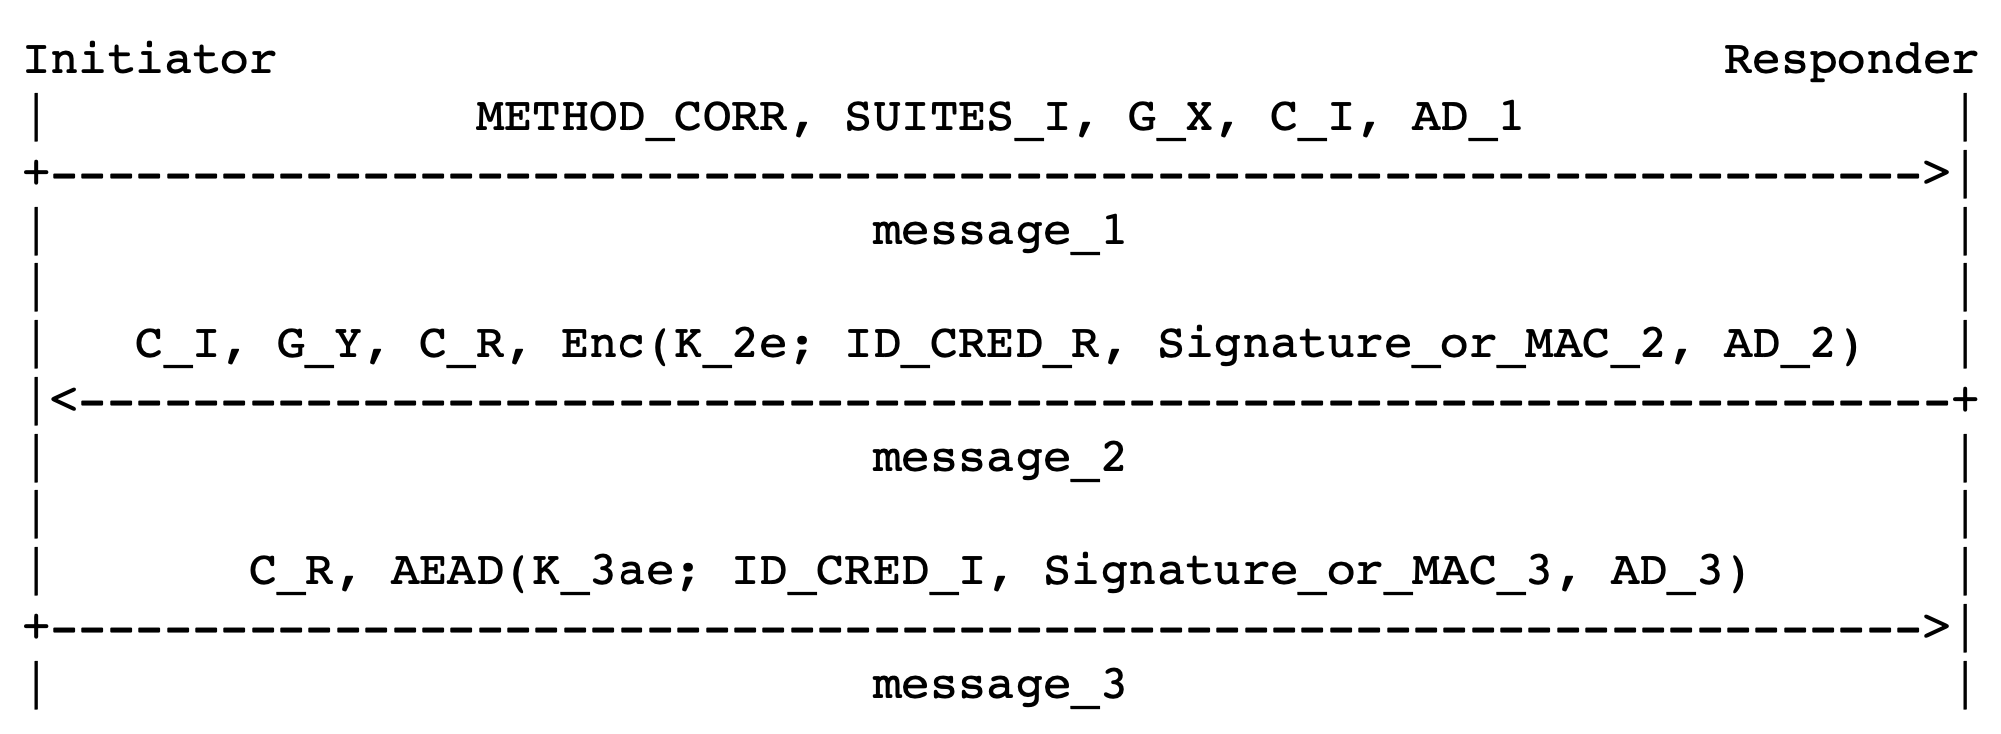
\includegraphics[scale=0.3]{Images/asym.png}
\scalebox{.7}{
\tikzset{>=latex, every msg/.style={draw=thick}, every node/.style={fill=none,text=black}}
\begin{tikzpicture}
    \node (ini) at (0, 0) {Initiator};
    \draw [very thick] (0, -0.5) -- (0,-13.3);
    \draw [very thick] (9, -0.5) -- (9,-13.3);
    \node[below=0.5em of ini,fill=white] {$
    \begin{array}{c}
    \text{Knows}\ $g$,\ \mCredi,\ \mLtki,\ \mIdcredi,\
    \mIdcredr,\ \mADone,\ \mADthree
    \end{array}
    $};
    \node (res) at (9,0) {Responder};
    \node[below=0.5em of res,fill=white] {$
    \begin{array}{c}
    \text{Knows}\ $g$,\ \mCredr,\ \mLtkr, \ \mIdcredr,\
    \mIdcredi,\ \mADtwo
    \end{array}$};
    \action{3.5em}{ini}{Generates \mMethod,\ \mSuites,\ \mCi,\ $x$\\$\mGx = g^{x}$};
    \msg{8em}{ini}{res}{\mMsgone: \mMethod, \mSuites, \mGx, \mCi, \mADone};
    \action{8.5em}{res}{$
      \begin{array}{c}
        \text{Generates } \mCr,\ $y$\\
        \mGy = g^{y}, \ \ \ \mGrx = \mGx^{\mLtkr} \\
        \mTHtwo = \mHash(\mMsgone, \langle \mCi, \mGy, \mCr \rangle)\\
        \mPRKtwo = \mHkdfExtract(\textrm{``\phantom{}''}, g^{xy}) \\
        \mPRKthree = \mHkdfExtract(\mPRKtwo, \mGrx) \\
        \mKtwom = \mHkdfExpand(\mPRKthree, \mTHtwo) \\
        \mMactwo = \mAead(\mKtwom; \langle \mIdcredr, \mTHtwo, \mCredr, \mADtwo \rangle; \textrm{``\phantom{}''}) \\
        \mKtwoe = \mHkdfExpand(\mPRKtwo, \mTHtwo)
      \end{array}$};
    \msg{21.7em}{res}{ini}{\mMsgtwo: \mCi, \mGy, \mCr, $\overbrace{\mKtwoe\ \mXor\ \langle \mIdcredr, \mMactwo, \mADtwo \rangle}^{\mCipher}$};
    \action{22.5em}{ini}{$
      \begin{array}{c}
        %\mTHtwo = \mHash(\mMsgone, \langle \mCi, \mGy, \mCr \rangle) \
        \mPRKtwo = \mHkdfExtract(\textrm{``\phantom{}''}, g^{xy}) \\
        %\mKtwoe = \mHkdfExpand(\mPRKtwo,\mTHtwo)\\
        \mGrx = \mCredr^{x} \\
        \mPRKfour = \mPRKthree = \mHkdfExtract(\mPRKtwo, \mGrx) \\
        %\mKtwom = \mHkdfExpand(\mPRKthree, \mTHtwo) \\
        \mKthreeae = \mHkdfExpand(\mPRKthree, \mTHtwo) \\
        \mTHthree = \mHash(\mTHtwo, \mCipher, \mCr)\\
        \mKthreem = \mHkdfExpand(\mPRKfour, \mTHthree) \\
        \mMacthree = \mAead(\mKthreem; \langle \mIdcredi, \mTHthree, \mCredi, \mADthree \rangle; \textrm{``\phantom{}''}) \\
        \mSigthree = \mSign(\langle \langle \mIdcredi, \mTHthree, \mCredi, \mADthree \rangle, \mMacthree \rangle, \mLtki)
      \end{array}$};
    \msg{34.5em}{ini}{res}{$\mMsgthree: \mCr, \mAead(\mKthreeae; \mTHthree; \langle \mIdcredi, \mSigthree, \mADthree \rangle$)};
    \action{35em}{res}{$
    \begin{array}{c}
        \mTHthree = \mHash(\mTHtwo, \mCipher, \mCr)\\
        \mKthreem = \mHkdfExpand(\mPRKthree, \mTHthree) \\
        \mKthreeae = \mHkdfExpand(\mPRKthree, \mTHthree)
    \end{array}$};
    \draw [line width=1mm] (-2,-13.3) -- (2,-13.3);
    \draw [line width=1mm] (7,-13.3) -- (11,-13.3);
    \end{tikzpicture}
}
    \caption{The \mSigStat{} method; (\mCredi{}, \mLtki), and
        (\mCredr{}, \mLtkr{}) are public-private key pairs; $\mSign(k, x)$
        denotes the signature of message $x$ using key $k$, and
    $\langle\cdot\rangle$ denotes a tuple. The hash function \mHash{} is the one
indicated in \mSuites{}.}
\label{fig:edhocsigstat}
\end{figure}
%------------------------------------------------------------------------- sub

The \mStatSig{} method mirrors \mSigStat{}.
%
The responder runs \mSig{} and creates \mAuthr{} as a signature over MAC, 
while the initiator runs \mStat{}.
%
%This is illustrated in Figure~\ref{fig:edhocstatsig}. 
This can be found in Figure~\ref{fig:edhocstatsig} in the appendix.
%
Finally, in \mStatStat{}, both parties use \mStat.
%Both parties' secret static long-term DH keys feed into the key schedule.
%%
%The initiator computes authentication data using the \mAead{} transform
%and includes that in the third message for the responder to verify.
%
%As expected, the initiator's behavior mirrors the \mStat{} authentication method used by the responder in \mSigStat{}.
%
%
% 
%\subsubsection{\mSigSig{}.}
%Both parties run \mSig{} and authenticate with signatures.
%%
%As mentioned earlier, \mSigSig{} is very closely modeled on \mSigmaI{}, but
%there are some notable differences.
%%
%For example, \mEdhoc{} aims to provide some degree of identity protection for
%responders, and therefore uses the idea from \mSigmaI{} of encrypting the
%responder identifier \mIdcredr{} (and other items) in the second message.
%%
%The designers of \mEdhoc{} consider it wasteful adding a second MAC in addition
%to the already included \mMactwo{}, to limit bandwidth consumption.
%%
%\mEdhoc{} applies XOR encryption, with \mHkdf{} being used to generate the
%key stream, whereas \mSigma{} assumes authenticated encryption for this
%purpose (see Section 5.2 of~\cite{sigma}).
%%
%Because \mSigSig{} has been analyzed in~\cite{DBLP:conf/secsr/BruniJPS18}, we
%do not focus on it here.
%%
%However, we model it and verify its properties as carefully as for the other methods.
%
%
%%KARL: we didn't verify anything about this after all. Propose to delete it.
%
%\subsection{Negotiating a cipher suite and method and correlation parameters}
%\label{sec:ciphersuite}
%Recall that we mentioned that the first message contains a list of cipher suites, ranked according to the preference of the initiator. What does a cipher suite actually contain? An \mEdhoc{} cipher suite consists of an ordered set of \mCose{} algorithms: an \mAead{} algorithm, a hash algorithm, an ECDH curve, a signature algorithm, a signature algorithm curve, an application \mAead{} algorithm, and an application hash algorithm from the \mCose{} Algorithms and Elliptic Curves registries.  
%
%There are four supported cipher suites in \mEdhoc{} -- we refer the reader to Section 3.4 of~\cite{selander-lake-edhoc-01} for the specifics of the algorithms allowed therein. Each cipher suite is identified by one of four predefined integer labels (0--3). Some algorithms are not used in some methods.  The signature algorithm and the signature algorithm curve are not used in methods without signature authentication (i.e. in \mPskPsk{} and \mStatStat).
%
%In order to keep the presentation clean, we have omitted the cipher suite negotiation process from the description of the methods. However, this process happens as follows, at the beginning of every method, once the responder receives the first message. The initiator proposes an ordered list of cipher suites they support. This list presented in descending order to the responder who either accepts the topmost entry in this list (if they also support that suite) or makes a counter-proposal, namely the topmost entry which they support from the remaining part of the list. If there is no such entry the responder can reject, and the protocol does not continue. Similarly, the responder can reject the initiator's choices for the method and correlation parameters as well -- in the case of a reject for either of these values, the protocol aborts.
%------------------------------------------------------------------------- sub
%\subsection{Claimed Security Properties}
%\label{sec:claimedProperties}
 %
%The \mEdhoc{} \mSpec{} \cite{selander-lake-edhoc-01} claims
%that \mEdhoc{} satisfies many security properties, but these are imprecisely
%expressed and motivated.
%%
%We will revisit these claims later. %when we discuss the formal modeling and
%%verification of \mEdhoc{}.  in Section~\ref{sec:formalization} and in the
%%discussions in Section~\ref{sec:discussion}.
%%
%%The following are our interpretations of the properties listed in Section~8.1 of \cite{selander-lake-edhoc-01}:
%\begin{itemize}
 %   \item Perfect Forward Secrecy (\textbf{PFS}) for the session key material
 %   \item Mutual (entity) authentication, followed by claims of
 %       \textbf{consistency}~\cite{sigma},
 %       \textbf{aliveness}, and
 %       \textbf{peer awareness} to the responder, but not to the initiator
 %   \item \textbf{Identity protection} (the initiator against active attacks
 %       and the responder against passive attacks, except for \mPskPsk{})
 %   \item Key Compromise Impersonation (\textbf{KCI}) resistance
%%    \item A single session of \mEdhoc{} enables the responder to verify
%%            that the selected cipher suite is the most preferred of the
%%            initiator which is supported by both parties, even though there is
%%            no negotiation of cipher suites per se.
 %   \item \textbf{Session key independence}
%\end{itemize}
